\chapter{Scalable User-centric cloud networking}
\ifpdf
    \graphicspath{{Chapter3/Chapter3Figs/PNG/}{Chapter3/Chapter3Figs/PDF/}{Chapter3/Chapter3Figs/}}
\else
    \graphicspath{{Chapter3/Chapter3Figs/EPS/}{Chapter3/Chapter3Figs/}}
\fi

% In this chapter we explore application of the SDN technology in Cloud Computing.
% The availability of cheap cloud computing resources, boosted the development of
% a wide ecosystem of applications that aim to fulfil the needs of users to handle
% efficiently and ubiquitly personal information.  We term this use case of cloud
% computing as Personal Cloud. Applications like facebook,
% dropbox, google services~et.al.  abstract online user identity among devices,
% associate it with information, which is disseminated based on the user policy.
% Such services manage to simplify the way we use computers, but most of the times
% they employ mechanisms that undermine the security and privacy of users, while
% use network resources inefficiently. 

In this chapter we explore applications of network control distribution in Cloud and
Mobile computing. The work focuses on the problem of information control and
distribution between the devices of a user across the Internet; a mechanism we
term Personal Cloud.  We propose \signpost, an Internet-wide overlay network architecture
that establishes Personal Cloud functionality and provides continuous connectivity
and controlled security. The architecture consists of daemons running on
end-user devices, which can configure and run several off-the-self connection
establishing software packages.  The proposed architecture employs a distributed
negotiation protocol between end-hosts, which scales the control complexity
through control distribution.

% The architecture provides two points of integration with legacy applications. 
% From the user perspective, the system integrates functionality on the
% network layer of the OS, thus providing backward compatibility with existing
% applications on the forwarding path. Additionally, the design provides a 
% user-friendly naming abstraction to devices, over the DNS protocol. DNS
% lookups for device names establish an API for applications to request from 
% the system the establishment of a path between 2 devices; a mechanism which we
% call {\it ``Effectful Naming''}.

% The propose architecture utilizes \of-enabled bridge and a
% local controller on each device. Each controller by default forwards packets as
% normal on the local network. The forwarding logic, though,  is augmenting
% through a distributed coordination protocol which permits nodes to negotiate
% possible connection opportunities and establish ad-hoc tunnels, enabling as a
% result an Internet-wide distributed control mechanism. 
% At the core of
% our design, we  the naming service host abstraction. Each device
% acquires a global domain name, while each name resolution triggers a connection
% engine, that tries to find the best possible bidirectional channel between the
% two nodes. The naming service uses the established
% DNSSEC extension, providing a fully authenticated and secure control
% mechanism among \signpost and applications. Further, the distributed nature
% of the naming hierarchy in the Internet permits seamless control distribution.

In order to understand the feasibility and performance of the proposed
architecture we develop a strawman implementation, which implements the core
control logic of the proposed architecture.  Additionally, it integrates support
for a number of network connection and notification services.  Currently,
\signpost supports SSH, OpenVPN, TOR, NAT-punch and Privoxy connection
mechanisms, while it can propagate Multicast-DNS notifications across devices.

In this chapter, we present in Section~\ref{sec:signpost-introduction} the
motivation for this work, followed then by the key observations for our design
in Section~\ref{sec:signpost-design}. In
Section~\ref{sec:signpost-architecture}, we present the architecture of our
strawman implementation and its integration with existing software. Finally, in
Section~\ref{sec:signpost-evaluation} we present a number of micro-benchmark
tests for our system and conclude in Section\ref{sec:signpost-conclusion}.

\section{Personal Clouds}\label{sec:signpost-introduction}

In the recent years, the increase in the number of computing devices per user
has created a significant information and resource management problem for
end-users. In this modern era, the ensemble of the user digital footprint
quantums establish a user's abstract digital presence. For example, a users work
facet comprises of his work documents and files, while a part of his social
experiences can be maps to his collection of digital photos. This digital
information is trated by the user as a single entity that he wishes to access
through any point of interaction with the digital domain.  Unfortunately, the
set of personal devices through which a user interacts with his digital presence
is large and consists on average of a laptop, a desktop, a tablet, a smartphone
and a number of low cost computational units for home entertainment and gaming.
These devices tend to offer specific user services and fulfil specific roles,
thus requiring access only to a subset of the user digital presence, but these
roles are fluid and intercept. For example, a smartphone is primarily a
communication device, while a number of end-users use smartphones to play audio
and video content. In the latter case, the smartphone and the home entertainment
system provide similar functionality to the user, require access to the same
subset of his digital presence and the user requires a simple abstraction that
can replicate his digital footprint between his devices, a functionality which
we describe as a \emph{Personal Cloud}. 

In order to address these requirements numerous applications and protocols have
been introduced that provide functionalities such as remote desktop access, file
sharing, remote login, remote printing etc.  between devices.  Such applications
extend existing computer abstractions and integrate mechanisms that allow user
to access information or resources between devices.  Additionally, the network
community has developed a number of mechanisms to reduce the configuration
burden of resource sharing mechanisms.  Multicast-DNS, Universal Plug and Play
and ZeroConf protocols allow a user to seamlessly browse and access available
shared services upon connection to a network.  Such mechanisms have managed to
improve significantly the digital experience in small scale network
environments, like the home network, but they face significant difficulties to
scale in heavily policed networks or across the Internet. In the rest of this
Section, we discuss the problems arising in Personal Cloud functionality over
the Internet~(Subsection~\ref{sec:sp-challenges}), present existing approaches
to the problem~(Subsection~\ref{sec:sp-approaches}) and introduce readers to the
\signpost framework~(Subsection~\ref{sec:sp-interface}).

% We term {\it ``Personal Cloud``}, the resource sharing and control abstraction
% that the user can exercise among his devices. Personal cloud is an efficient way
% for users to embrace technology and take full advantage of it. Unfortunately,
% interconnecting devices across the Internet has become increasingly difficult.

% , mainly due to the
% way that the Internet evolves.

\subsection{Challenges} \label{sec:sp-challenges}

Internet is an excellent example of a dynamic system managing to address
effectively evolution.  In the early days of the system, in
order to extend user adoption, its  steering committee set simplicity and
openness as two fundamental design goals. Due to these design choices, Internet
protocols gained rapidly support by a wide range of OSes, while the set of
connected entities augmented exponentially.  Nonetheless, during that period, the
Internet remained a large wide area network, interconnecting research
institutes, and the predominant applications provided constraint relaxed
asynchronous communication. Through the years though, and as Internet users
increased, new applications emerged and highlighted a number of
security and performance limitation in the initial design of the system.

In order to address these limitations in a backward compatible manner, a number
of network hacks were introduced in the Internet design. One of the most popular
hack is the deployment of middleboxes~\cite{RFC3234}.  Middleboxes violate in a
number of ways design principles of the Internet, in order to provide an effective
framework to ``inject`` functionality that addresses design limitation. For
example, 
\emph{NATboxes} handle the IPv4 address space shortage, \emph{WAN optimizers}
improve utilization of under-provisioned links, while \emph{firewalls} secure
critical networks.  Unfortunately, Middlebox deployment redefines to a great
extend the Internet abstraction. A number of papers have described their
impact: in~\cite{Honda:2011ci} authors pinpoint middlebox functionality as a
core cause in the ossification of the transport layer, while
in~\cite{Kreibich10} authors describe a wide range of protocol functionality
that has
become suppressed due to middlebox functionality. 
% Mainly, due to middlebox functionality, the
% initial design properties of the system in terms of simplicity and openness have
% been lost for a large subset of the Internet.  

\todo{ describe some efforts to overcome middleboxes.}
\todo{IPv6 can do some of that,but not everything }
An important impact of middlebox deployment is the reduced connectivity
introduced in the Internet. Home networks host a number of hidden devices which
remain inaccessible from the Internet due to NATbox functionality, while strict
firewall policies in enterprise networks reduce protocol functionality.
Personal Cloud deployment across the Internet is increasingly restricted, as
devices are not able to interconnect directly.

% §develop and deploy various protocol modifications that tried to bypass these
% design flaws.  Unfortunately, such systems tend to introduce stricter
% assumptions on how the network should function, and reduce to a great extend the
% openess of the Internet.There are primarily two major classes of engineering
% modifications that reduce network connectivity: performance enhancing
% middleboxes and edge-network security policy reinforcement.  
% Performance
% enhancing middleboxes are network forwarding devices, installed in the network,
% that aggregate information from multiple layers of the TCP/IP stack and modify
% packet content or forwarding logic. 
% This restriction in openess of some parts of
% the Internet is a vital reason for the inability of the network community to
% establish Private Clouds across the Internet.  

\subsection{Approaches} \label{sec:sp-approaches}

% Although reachability is reduced, Internet remains a highly performant and
% connected system; it interconnects billion of users and transports Terrabytes of
% information daily. This is achieved due to the predominant operational model of
% Internet services. Hosts in the common case connect to a small subset of the
% Internet space that provides access to popular information.  This model, which
% is called {\it Client-Server model}, is a natural result of the power-law
% chatacteristics of various social and engineering mechanisms. Internet network
% graph is a power law graph, due to its scalable hierarchical structure, while
% information popularity exhibits strong power law characteristics. 

Personal cloud computing requirements currently experience a mismatch with the
functional properties of the Internet.  Personal devices usually connect to networks
optimised for outgoing connectivity and various components of the
Internet are not designed to accommodate well-connected services for every host.
NATed networks, that scale connectivity on the edges of the network, require
manual configuration in order to host Internet-reachable services, while a
number of edge networks, namely mobile and enterprise networks, restrict
publicly accessible services on connected hosts for security reasons. In order
to overcome these restrictions a number of approach has been proposed by the
research community, as well as the industry.  We group these solutions in the
following two categories:

\paragraph*{Decentralised Personal Cloud}: 

Numerous frameworks have been proposed over the years that enable bidirectional
connectivity between devices, using publicly available Internet resource. We are
considering in this category tunneling software, like OpenVpn and SSH, and NAT
and firewall punching mechanisms, like STUN. Although such mechanisms are
effective in a number of scenarios, assumptions and configuration requirements
dim them inappropriate for inexperienced users. As we have already discussed in
Section~\ref{s:home_social}, average Internet user is highly improbable to
engage in systematic network configuration, if the configuration tasks are long
or complex. Establishing connectivity through user-managed mechanisms is not
straightforward or guaranteed to succeed. Functionality contains assumptions on
the connectivity of the environment and users have to resolve to ``try and
error'' approaches to check which mechanism can be effective in a specific
environment, while a number of different network subsystems require prior
configuration. 

As an example, we describe the steps required by a user to establish
connectivity using the SSH service. Before the user is able to connect to a
computer using SSH, he has to configure the service on his local machine, the
security credentials on the server and any firewall and NATbox deployed in the
network. Additionally, if his public IP is expected to change over the course of
a day, he needs to setup a mechanism to access the current IP configuration,
like DynDNS.  During connection establishment, the user has to run the SSH
client, configure the ports he is interested to forward and configure the
connecting software to use them.  This connectivity is subject to the ability of
the user in the remote network to use the SSH protocol on the preconfigure port.
In case this is not possible, the user has to resolve to a different service.

\paragraph*{cloud-assisted Personal Cloud}:

% According to wikipedia~\cite{wiki-cloud}, the definition of {\it ``Cloud''} is:
% \begin{quote}
%   Cloud computing is the use of computing resources (hardware and software) that
%   are delivered as a service over a network (typically the Internet). 
% \end{quote}
% The {\it``Coud''} has been a buz world that receive increased attention within
% the recent years.  The concept is not novel for the computer science community,
% and can be placed under the generic engineering technique of abstraction and
% virtualisation. Its popularity though can be mapped to theeffectiveness of the
% abstraction as well as the increased interest in distributed large data
% processing infrustructure.  Interestingly, the initial idea for cloud computing
% aimed to create a small scale economical market that would take advantage of
% iddle data center resources, but the model became so successful that companies
% create new data center infrustructure solely to support this service. 

% Our work in this chapter aims to revisit the design of cloud applications that
% target end-users and provides them the ability to store and share
% information. Such application usually consist of 2 layers of abstraction, which
% oftenly are not controlled by the same entity. In the lower layer of the system
% we find the infrastructure abstraction layer, which is usally termed as
% {\it Infrustructure as a Service}. This service is controlled by the
% entity that controls the data center and ensures and enforce the required resource
% allocations over the available hardware. Usually, this relies on the management
% of a large number of commodity servers running an OS virtualisation framework,
% like Xen, and configure the network in order to match the resource
% virtualization mechanisms. At the upper layer of the system, we find the service
% abstraction layer, which is also called as the {\it Software as a Service} or
% {\it Platform as a Service}. This layer provides the resulting abstraction to
% the user, and it main focus is to translate the required functionality
% by the user into a number of distributed computations that can be distributed
% over the abstraction of machines that the lower layer provides. In most of the
% cases, the end-user of a cloud application is usually exposed  directly only to
% the upper layer of the afortmentioned abstractions. 

% Cloud computing mechanisms have managed to provide a sufficient platform that
% can accomodate the processign requirements for a large number of applications,
% while it also provides ways to scale systems very fast in order to support
% emerging applications. The main architectural approach that has been used in
% order to achieve is to direct users to a centrally controlled system. User copy
% their data to the public cloud infrustructure and interact with the public API
% of the service. The service provider can post analyse the user data in order to
% create the intermediate data required in order to provide timely responsiveness
% for its service.

An alternative approach, which has been highly successful in the recent years,
uses third party services to establish inter-device connectivity.  In this class
we consider cloud applications like the Google service suite and Dropbox. These
applications provide a simple, intuitive and ubiquitous mechanisms to store and
retrieve data in the cloud and define information dissemination policies.
Although this approach can be characterised as successful in providing the
required functionality, some of the properties are ambivalent and demotivate
user engagement. 

\begin{itemize}
  \item{\it authentication}: Cloud applications provide an effective control
       framework to disseminate information between devices and users.  Users
       define access policies based on online identities and the service ensures
       secure information delivery.  User authentication mechanisms though
       introduce privacy concerns, since they can be employed to identify and
       monitor users.  In~\cite{Krishnamurthy2009} authors reports cases of
       personal information leakage to ad services from Online Social Networks,
       in order to detect and characterize individuals, and Facebook has openly
       verified the existence of such
       services~\footnote{\url{http://en.wikipedia.org/wiki/Facebook_Beacon}}. 

% \paragraph*{authentication}: A number of cloud applications provide an effective framework
% to control information dissemination between devices as well as users. 
% Users are required solely to verify that an online identity is a valid destination for
% an information quantum. The platform will ensure that the information will be
% accessible only to users that have the valid credentials for that account in any
% time, easing the information access control from end-users. This mechanism has
% been further used by other application to offload their authentication mechanism
% to a third party cloud service. This mechanism though has been reported to be
% abused by some service providers. In~\cite{Krishnamurthy2009} authors reports
% cases of online OSN that leak information to ad services which allows them to
% detect and characterize individuals. This was recognized by facebook as a paid
% service provide to ad services and removed after wide privcacy concerns by
% users~\footnote{\url{http://en.wikipedia.org/wiki/Facebook_Beacon}}. The wide
% adoption of such authentication mechanisms raises concerns for the control of
% the privacy of users.  
% On the other hand though, it has been reported that some cloud
% applications have engaged in leaking information on users to third party
% application. A study in~\todo{add reference} reports that the social network
% facebook leaks identity hints to advrtising platforms in order to enhance their
% ability to characterise users, a functionality which is privacy envasing for
% some users. 

\item {\it performance}: The availability of large amount of computational
      resources in current cloud infrastructures provide user acceptable
      performance, regardless the volume of processed data.
      This approach though under-utilize the rich computational resources 
      available in 
      end-users device on the edges of the Internet.  Two devices connected to the
      same subnet will experience bloated RTT values when they communicate
      through a cloud service, while public cloud storage cost and performance
      is orders of magnitude worse than local network file services.
      In~\cite{Wittie2010}, authors report a significant impact on the 95th
      quantile network performance of cloud services, due to latency and packet
      losses incurred by the Internet.
      \todo{Add dropbox measurement study}
% \paragraph*{performance}: A number of cloud services manage to deliver user
% acceptable performance to million of users across the world. This is achieved to
% a great extend by careful design of data processing pipelines, that paralelize
% processing logic and preemptively calculate results for future user requests.
% Additionally, large service providers develop global distribution networks with
% multiple entry points close to the user.  Google claims that any user is in
% range of a few thousand of mile of at least a signle google datacenter. Although
% this approach provides a user satisfying service performance, it is wasteful in
% processing resources; Cloud services under utilize rich edge resources. Two
% devices that are behind the same subnet and communicate using a cloud service 
% have to communicate through the datacenter infrustructure of the provider, 
% increasing significantly latency. Additionally, public cloud storage cost is two
% orders of magnitude more expensive that the cost to maintain data on your local
% disk. 
% Finally, a number of measurement studies have highlighted a significant impact
% on the 95th quantile performance of cloud services, due to latency and packet
% losses incurred by the Internet~\cite{Wittie2010}. 

\item {\it cost}: Free cloud services employ a 3-party economical model that
      subsidizes infrastructural costs through advertisement. Nontheless, 
      cloud services, due to the free nature of the service, provide very weak SLA's. If
      a part of the service is compromised and sensitive information is leaked,
      the service provider bears minimum obligation towards affected users. Such
      costs are not directly observed by the end-user, but they may impact
      significantly his social and work experience. 
      \todo{report Dropbox problem}
% \paragraph*{cost}: Free cloud services have an interesting 3-party economical
% model that uses advertisment as a mechanism to circulate capital and sustain the
% cost of the infrustructure. As a result, users are able to enjoy high quality
% services with minimum costs. The SLA's though, because of the free nature of the
% service are not wiling to provide any SLA's to users. If a part of the service
% is compromised and some information is leaked, then the service provider bears
% no obligation towards affected users. Such costs are not directly observed by
% the end-user, but they may impact significantly his everyday life. 

\item {\it Availability}: Cloud services run on well connected infrastructures
      with a large number of network engineers ensuring security and
      performance. Any device with Internet connectivity is able to connect to
      the cloud service without any network configuration.  This centralisation
      of the services over the Internet, introduced a weak link in the service
      functionality. Devices that can connect directly over a network, 
      will never be able to interconnect and exchange information, if Internet
      connectivity is unavailable.  Two users behind the same firewall will never be able to
      exchange a file over Dropbox, if the network policy forbids any connection
      with the servers of the service. 
% \paragraph*{Availability}: As we have already discussed in the Introduction of
% this thesis, Internet has reduced significantly the bidirectional connection
% property of Internet hosts. The deployment of performance-enhancing middleboxes
% makes highly impossible for a device to expose an Internet-wide service.
% Additionally, the large number of malicious nodes that try to exploit security
% vulnerabilities, is counter intuitive for users. Cloud service providers address
% this problem in a highly effective manner. Their network default policy is
% permit, while a handful of network engineers are constantly monitoring the
% security of the datacenter and ensure high availability of the system and data
% integrity.  As a result, any device with Internet connectivity is able to
% connect to the service, without any special configuration of the OS or the
% Network policy. Cloud services function as a proxy between devices and users,
% that provides them connectivity in most cases. Although, the centralised
% design of such services makes it impossible for devices to interconnect when
% there isn't any Internet connectivity. Two users behind the same firewall will
% never be able to exchange a file over dropbox, if the network policy forbids
% any connection with the servers of the service. 
\item {\emph Generality}: Cloud applications develop distributed services
      optimized for specific functionality. Google Drive provides online
      document storage, Youtube provides online video hosting and Facebook
      provides Online Social Network Services. Users are limited on their ability
      to share information or resources by the offered capabilities of the
      service provider and there isn't a sole service provider that can
      support functionality for the complete ensemble of Personal Cloud services. 
\end{itemize}

\subsection{Reconnecting the Internet}\label{sec:sp-signpost}

\signpost is a Personal Cloud enabling framework with user controlled security.
The system establishes an Internet-wide overlay network between the devices of a
user, combining the aforthmentioned approaches. The abstraction relies on a
cloud-based control channel established between devices which can be used to
negotiate and establish highly efficient end-to-end connections, using existing
decentralized frameworks. In order to ensure functionality
under any circumstance, we integrate the control channel with the DNS protocol, a highly
available and resilient service. 

\signpost has two major design goals.  Firstly, the system establishes a user
friendly framework that automates end-to-end path configuration between devices.
\signpost models the way various existing decentralised mechanisms establish
connectivity and encode their configuration and assumption testing in a generic
automation framework.  Additionally, the system seamlessly integrates support
with existing applications. \signpost network paths are exposed in the network
layer of the OS, while the API to control the establishment of connection is
integrated with the \textit{gethostbyname()} function.  Each device is exposed to the users as a
domain name and a name lookup for a device triggers the connection establishment
mechanism, while traffic send to the returned IP is forwarded through \of over
the established path.  Secondly, the system exposes a user-controlled security
abstraction, which can provide different security properties on connections
between devices. As a result, the user is able to fully control the
dissemination of information between his devices, while avoiding
privacy sensitive data offload to cloud services. 

\begin{figure}[ht]
  \begin{center}
	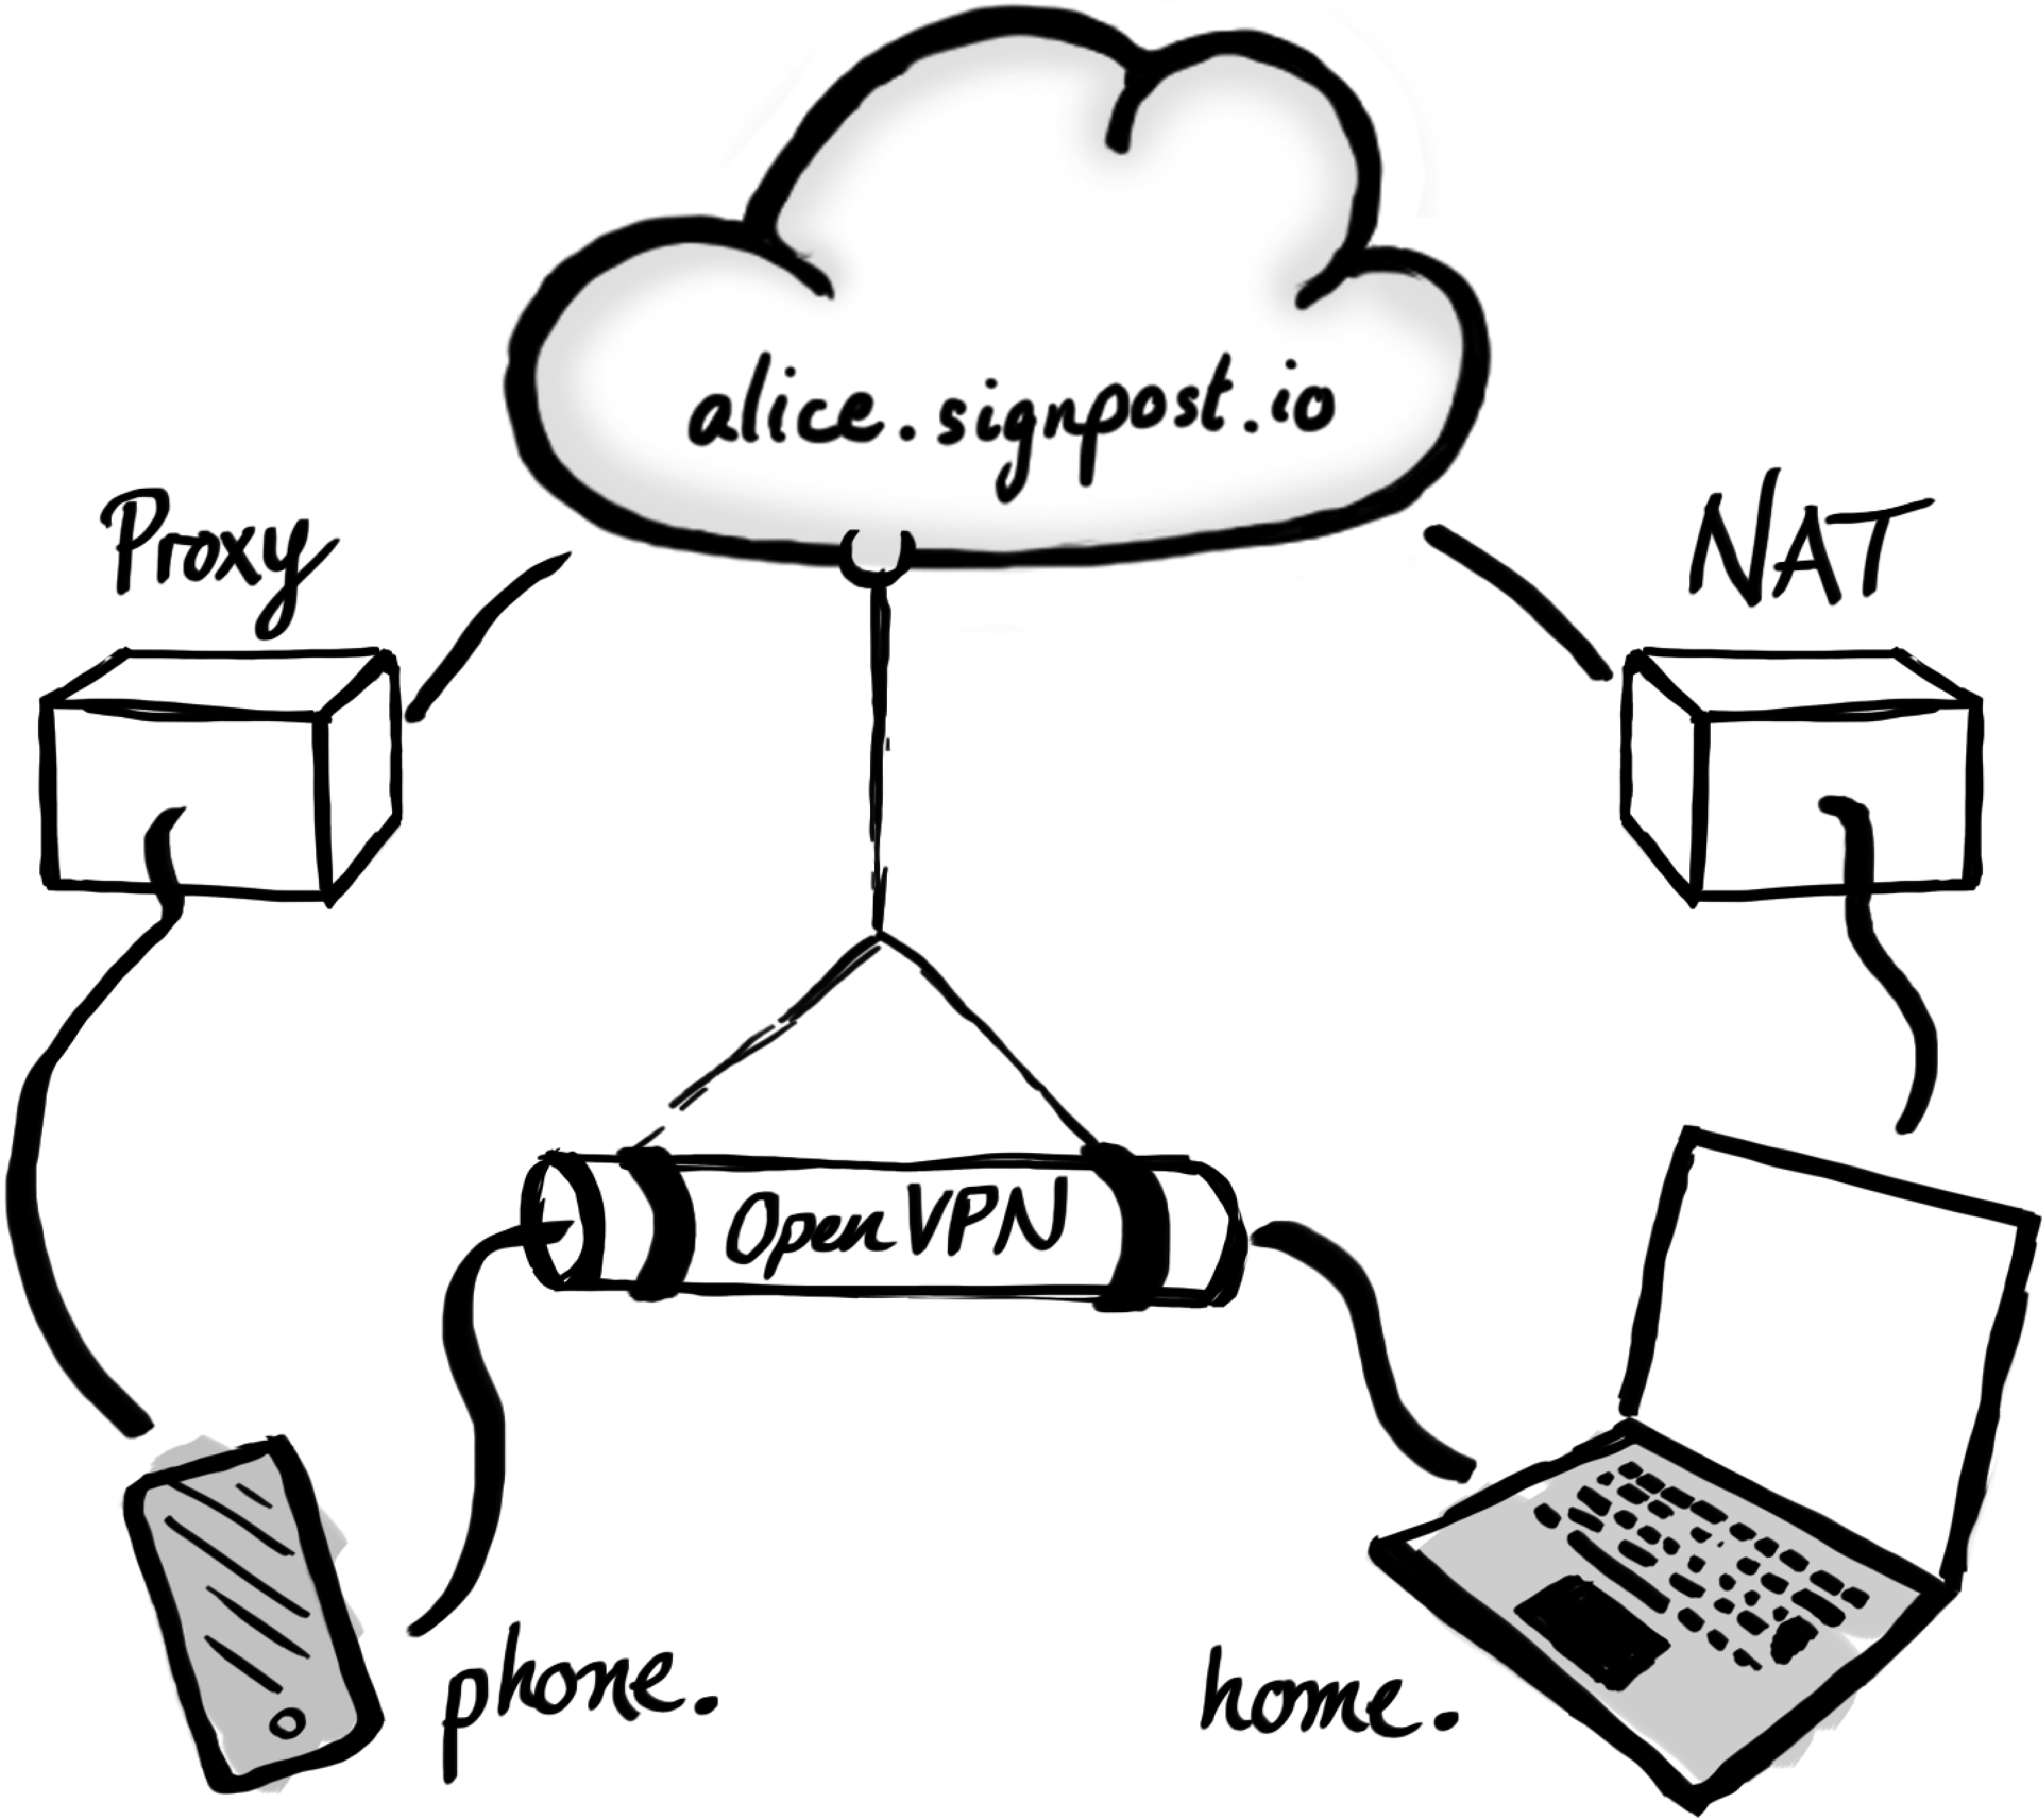
\includegraphics[width=0.6\textwidth]{signpost-illustration}
  \end{center}
  \caption{A simple example of the \signpost abstraction when the user Alice
    interconnects a smarthphone with the home computer over the Internet.}
  \label{fig:signpost-user-abstraction}
\end{figure}
\todo{Add some reference to cloud controller}
A schematic of the abstraction that our system provides to end-users is depicted
in Figure~\ref{fig:signpost-user-abstraction}. In this scenario user Alice, who
is at work and uses her smartphone, wishes to access some files on her laptop,
which is behind the NATed home router. In order to express her interest to
connect to her laptop, Alice needs solely to perform a name lookup for the
domain name \fqsn{laptop.alice}. The name lookup will propagate through the
DNS infrastructure to the cloud presence of her \signpost system. The \signpost
server will trigger the two devices to try multiple possible connection
establishment techniques and
setup an end-to-end path between the two devices. Once the server has
ensured that a first path is available, it will reply to the initial
DNS query with a local IP address which will be routed by the local network
stack to the tunnel between the two devices. In parallel, the server will
continue recursively to test different tactics, to discover more efficient
connection mechanisms. 

% Our work builds on the observations on the shortcoming of current approaches to
% interconnect devices, and tries to bridge the two domains, providing the
% appropriate control mechanisms to end-users. On one hand, we want to
% model a generic framework that will allow end-host to automatically test the
% network environment, discover the optimum mechanism to interconnect two
% devices and distributely negotiate the connection parameters with other devices,
% without any user interaction. On the other hand, we want to provide to the users
% a mechanism that will allow them to control to a great extend the security and
% privacy of their information. 

\section{\signpost Architecture}\label{sec:signpost-architecture}

\begin{figure}
  \begin{center}
	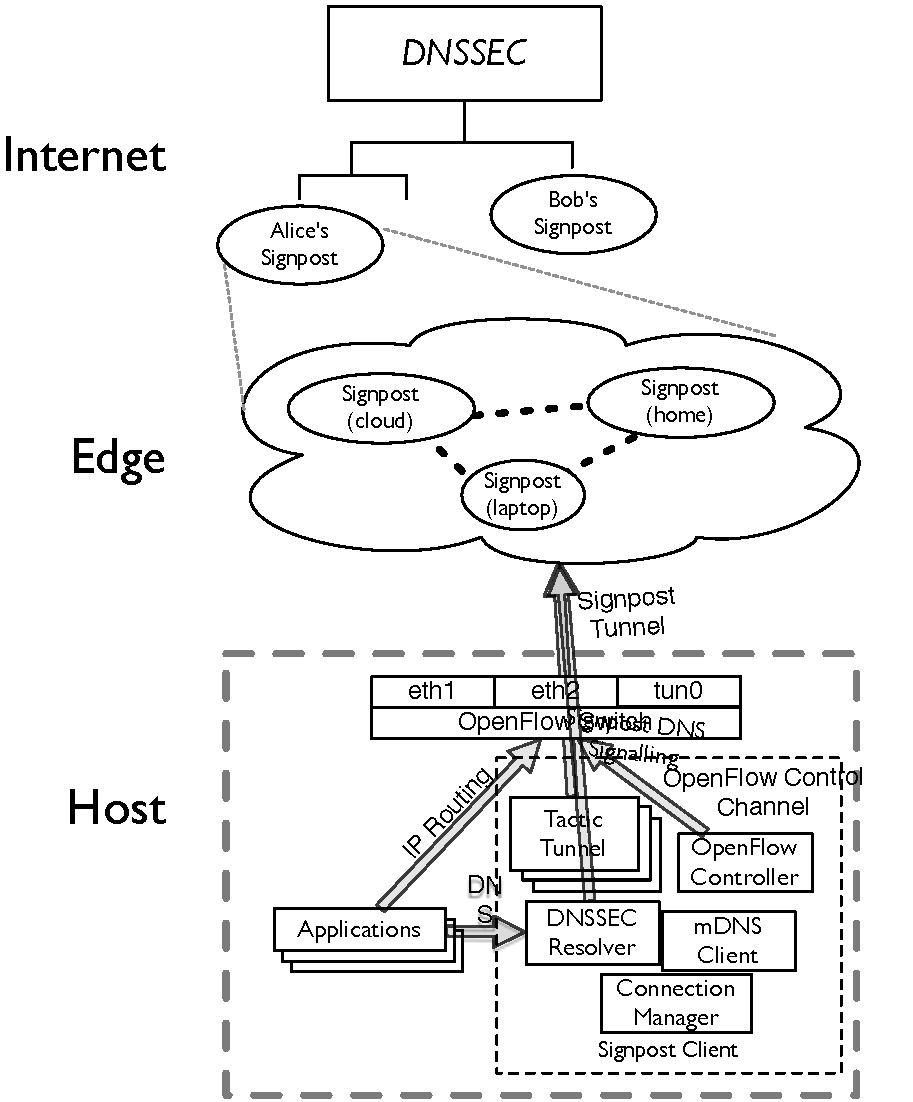
\includegraphics[width=0.9\textwidth]{signpost-arch}
  \end{center}
  \caption{\signpost architecture}
  \label{fig:signpost-arch}
\end{figure}

\signpost is an Internet-wide secure inter-device communication system. The
system reuses existing Internet protocols and connectivity mechanisms and provides
an overlay local network. In Figure~\ref{fig:signpost-arch} we present 
a diagram of the \signpost architecture over different abstractions. 
%%
In the lower section of Figure~\ref{fig:signpost-arch}, we present the design of
the \signpost software and its integration with existing applications.
\signpost logic is contained in a single executable, and requires from the guest
OS to expose an OpenFlow switch interface and redirect DNS queries to the
embedded DNS resolver.  The software consists of three main subsystems: A
{\it Connection Engine}~(Subsection~\ref{signpost-engine}) that sets up and
manages {\it Network Tactics}~(Subsection~\ref{signpost-tactic} in order to establish
end-to-end paths, a local DNS resolver and an \of-based {\it \signpost
  router}~(Subsection~\ref{signpost-forwarding}) that enhances the normal OS
routing functionality with \signpost logic.  
%%
In the middle layer of Figure~\ref{fig:signpost-arch}, we present the control
plane interconnection of \signpost devices. The system relies on an
Internet-wide inter-device control channel, which enables
connection capability and parameter negotiation. The architecture considers a
\emph{Controller \signpost} instance running on a well connected host, which bridges
the device control channel across the Internet.  Further, the system can
establish connectivity between local devices without the mediation of the
\signpost Controller.  \signpost clients contain a Bonjour-based discovery
mechanism, through which devices can establish ad-hoc secure and authenticated
paths.
%%
In the upper layer of Figure~\ref{fig:signpost-arch}, we present the naming
organisation of the \signpost architecture. The system reuses the naming
abstraction of the DNS service. Each device has a global domain name, while the
domain hierarchy and name aliasing expresses the control relationship between
devices and users.  We extend the normal name resolution functionality of the
DNS protocol and introduce the  {\it Effectful name resolution} operation for
\signpost-enable domains; a name resolution expresses the interest of a user to
establish an end-to-end path~(Subsection~\ref{signpost-naming}). For the rest of
the section we present in depth the details of the \signpost system. 

\subsection{Network Tactic} \label{signpost-tactic}

\begin{table*}
\centering \footnotesize
\begin{tabular}{|l|c|c|c|c|c|c|p{1.5cm}| }
  \hline
  Tactic name & Purpose & Layer & Transport & Auth. & Encrypted & Anon. & \signpost
Support\\
 %% & Comment & Source \\
\hline
Avahi       & Discover         & 7      & UDP         & No     & No     & No & Yes\\
 %% & Linux-based, bonjour-compatible system for local network resource discovery
 %% & \url{avahi.org/} \\
Samba       & Discover         & 7      & UDP         & No     & No     & No & No \\
 %% & Windows local network resource discovery protocol, implemented in WINS & \\
Bonjour     & Discover         & 7      & UDP         & No     & No     & No & Yes\\
 %% & Used for local network resource discovery
 %% & \url{developer.apple.com/opensource/} \\
Universal PnP & Discover         & 7      & UDP         & No     & No     & No & Yes\\
dns2tcp     & Tunnel             & 7      & UDP         & No     & No     & No & No \\
 %% & IP over DNS & \url{www.hsc.fr/ressources/outils/dns2tcp/index.html.en} \\
DNScat      & Tunnel            & 7      & UDP         & Yes    & No     & No & No \\
 %% & VPN with PPP & \url{tadek.pietraszek.org/projects/DNScat/} \\
HTTP-Tunnel & Tunnel            & 7      & TCP         & No     & No     & No & No \\
 %% & uses HTTP & \url{www.nocrew.org/software/httptunnel.html} \\
iodine      & Tunnel            & 7      & UDP         & Yes    & No     & No & Yes\\
 %% & IP over DNS & \url{code.kryo.se/iodine/} \\
NSTX        & Tunnel            & 7      & UDP         & No?    & No     & No & No\\
 %% & IP over DNS. Deprecated. Recommends iodine 
 %% & \url{thomer.com/howtos/nstx.html} \\
% IMAP        & Data transfer     & 7      & TCP         & Can be & Can be & No \\
 %% & & \\
Proxytunnel & Tunnel            & 7      & TCP         & Can be & Can be & No & No\\
 %% & can use both HTTP and HTTPS & \url{proxytunnel.sourceforge.net/} \\
ptunnel     & Tunnel            & 4      & ICMP        & Yes    & No     & No & No\\
tuns        & Tunnel            & 7      & UDP         & &        No     & No & No\\
 %% & IP over DNS. Doesn't split IP packets, but sets size so small that OS does
 %%   fragmentation. Neat. Only uses CNAME for maximum compatibility with
 %%   infrastructure. Poor performance :( 
 %% & \url{www.loria.fr/~lnussbau/tuns.html} \\ 
SSH         & Tunnel/Encrypt & 7      & TCP         & Yes    & Yes    & No & Yes\\
IPSec       & Tunnel/Encrypt & 3 (4*) & IP          & Yes    & Yes    & No & No\\
 %% & In layer 4 when traversing NATS (over UDP or TCP) & \\
OpenVPN     & Tunnel/Encrypt & 7      & UDP/TCP     & Yes    & Yes    & No & Yes\\
 %% & & \url{openvpn.net/} \\
libjingle   & Nat punch         & 7      & UDP/TCP     & Yes    & ?      & No & No\\
 %% & For punching holes. Negotiation over XMPP
 %% & \url{code.google.com/apis/talk/libjingle/index.html} \\
privoxy     & Anonymize         & 7      & TCP         & ?      & ?      & Yes & Yes\\
tor         & Anonymize         & 7      & TCP         & No     & Yes    & Yes & Yes\\
 %% & & \url{www.privoxy.org} \\
% SMTP        & Data transfer     & 7      & TCP         & Can be & Can be & No \\
stunnel     & Encrypt        & 7      & TCP         & Yes    & Yes    & No & No\\
TCPCrypt    & Encrypt        & 4      & TCP         & No     & Yes    & No & No\\
\hline
\end{tabular}
\caption{\label{tbl:signpost-tunnels}Tactics table.}
\end{table*}

Currently the network community offers a wide selection of software to establish
connectivity between network devices. In Table~\ref{tbl:signpost-tunnels}, we
present a small survey of such mechanisms along with their network requirements
and security properties.  From the data of the table, we note the high diversity
between connection properties. For example, a significant subset of the
mechanisms abuse application layer protocol functionality in order to establish
IP connectivity, thus allowing users to bypass strict network policies. An equally
significant subset of the mechanisms focus on encryption and privacy enhancement
of end-to-end Internet paths, while a third class of these
mechanisms enables connectivity through simple service advertisement. Further,
the mechanisms vary significantly on the network layer they operate and the type
of connection they provide.  Tunnels provide connectivity on a specific port of
the transport layer, or introduce an overlay network on the network layer.
The majority of the tunelling mechanism functions over UDP or TCP
protocol, while there are protocols that function over lower layer protocols, like
ICMP. Finally, authentication of users is not uniform.  Approaches vary from
user-based authentication, using either passwords or certificates, 
to simple passphrase checks, while a subset of the protocols doesn't
support any authentication. 

Due to the wide and diverse range of available mechanisms, we model their
functionality in terms of \signpost through a simple abstraction, which we term
{\it Network Tactic}. A sufficiently generic specification of this abstraction
is core for the establishment of an automated connectivity platform.
This abstraction enables modularization during the integration of new mechanism,
while enabling the development of algorithms that optimize specific indexes on
the exploration of the optimal combination of tactics to fulfil a user
connection policy.

\begin{figure}
  \begin{center}
	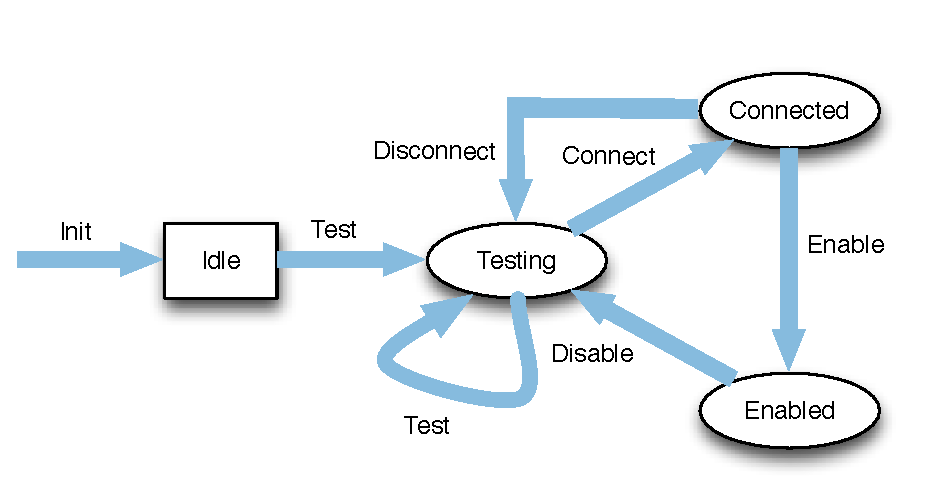
\includegraphics[width=0.6\textwidth]{signpost-tactic}
  \end{center}
  \caption{\signpost tactic lifecycle}
  \label{fig:signpost-tactic}
\end{figure}

Each tactic in \signpost is modelled as a 4 state automaton.  The state space
diagram is presented in Figure~\ref{fig:signpost-tactic}. A tactic is
initialized in the Idle state. A test method invocation transfers the tactic to
the testing state, while executing the testing logic of the tactic. The test
method performs tactic specific testing in order to detect the limitations in
network connectivity and the configuration required in order to establish
connectivity. If testing is successful, the tactic can progress to the connect
state which will configure an end-to-end path. Once the end-to-end path is
setted up, then the Tactic can progress to the enabled state and forward packets
to the end-to-end path.  Finally, the tactic automata provides methods to
backtrack from each state and clear stored state. In order to avoid packet
reordering, \signpost permits parallel existence of multiple connected tactics
for a set of devices, but a single tactic can be enabled at any point. 
\todo{ Mention that tactic is able to control OpenFlow also}

In term of modules implementation, \signpost achieves control distribution
through the definition of a generic model to split functionality between the
\signpost controller and client for a specific tactic.  The functionality of a \signpost tactic
is split logically in two layers: the Southbound layers, which implements low
level tactic operations, and the Northbound module,
which translates the tactic abstraction into low level operations.  The
Northbound module logic is executed by the \signpost controller, while the
Southmodule module logic is executed by the \signpost clients. The two layers of
the tactic, communicate over the control channel using a tactic specific
protocol. 

As an example of this functionality split, we present the Test methof of the
OpenVpn tactic, an IP tunneling system that uses certificate-based
authentication and functions over TCP or UDP. In the test section of the
Southbound layer, the tactic exposes two main functionalities: init an OpenVpn
server with default configuration and test if an OpenVpn server is accessible on
a given IP and port. The Northbound layer of the tactic will instruct all
devices participating to initiate a server instance and test connectivity to the
other end of the link. The first client that will return with a successful
result will become a client, while if the test request times out for both
devices, then the server will initialise an OpenVpn server and instruct the
devices to test connectivity through the cloud.

% In the development of the 
% we also consider the way that the
% design can encapsulate the complexity to address the problem of increased
% heterogeneity of the level of connectivity that a Network Tactic provides, we
% include two equally important details in the abstraction. Firstly, each tactic
% can directly modify the forwarding table of the OpenFlow Switch and receive
% feedback from the forwarding plane. In this way we can incorporate in the
% architecture tactics that provide port-based connectivity, as well as network
% layer connectivity. Secondly, because we are interested to allow user
% flexibility on the properties Tactic synthesis in order to enable complex
% combinations of Tactic that can fulfil user policy, we introduce in the design a
% simple mechanism to express meta-data informations on the connection
% requirements of a 

\todo{Discuss weight of tactics}

\subsection{Forwarding} \label{signpost-forwarding}

In order to add seamless \signpost support in existing applications we choose to
enable \signpost integration at the network layer. As a result, a \signpost
cloud is abstracted as a local subnet and persistent local IPs are allocated to
devices. In order to modify the forwarding logic of the end-host, we add a
requirement for an \of switch running on the local system which will be
connected to the embedded \of controller of the \signpost software. 

The forwarding logic of \signpost avoids any interference with the normal
network functionality of the system. \signpost is responsible to handle flows
that are under the \signpost local subnet and the system at start up configures
appropriately the routing table of the host, as well as the \of flow table of
the switch with static entries. For flows that interconnect \signpost devices
under the \signpost subnet, the system delegated their control to the respective
enabled tactic which can exercise control either actively or pro-actively
through a simple event driven model. Additionally, the controller enables
tactics to inject packets in the network, through the \of protocol, while they
are also able to install proactively \of flows that can modify normal network
routing functionality.
Tactic developers have to be careful with this control delegation and install
flows that affect solely tactic traffic. Finally, in order to reduce broadcast
traffic notification in the control channel, we implement a simple ARP cache as part of the \of
controller. The ARP caches replies with the MAC address fe:ff:ff:ff:ff:ff on
every ARP request for IP addresses within the \signpost subnet. Tactics are
responsible to exercise network level forwarding control. 

\subsection{Connection Manager} \label{signpost-engine}

\signpost is able to establish multiple end-to-end paths between devices through
tactic synthesis. Unfortunately, multipath connectivity is not supported by
popular transport protocols and newer protocols like SCTP and multipath TCP,
that support multipath connectivity, are not available in production applications.
Multipath functionality in \signpost could be integrated in existing transport
protocol through careful \of flow manipulation, but because performance is not
homogenous between paths,
packet reordering may occur and reduce network stack functionality.  As a
result,  \signpost we establish and use a single end-to-end path between any
two devices.  Path search
and establishment is encapsulated in the Connection Manager Subsystem. 

\signpost path selection mechanism considers two parameters: tunnel performance
and security policy. In terms of tunnel performance, we use a weight
mechanism and represent performance as a positive integer value, defined manually by the
developer. We use a set of simple rule of thumbs to define tactic performance
weight. Tactics that include the Controller in the forwarding path, are
considered less efficient than those establishing direct connectivity, while
tactics that run over connectionless protocols, like UDP, are preferred over
protocol that run over connection-oriented protocols, like TCP.  In cases of
tactic synthesis, the performance index is computed as the sum of the
performance of the partial tactic. This simplistic approach appears to be
sufficient at the moment, but more complex tactic specific mechanisms can be
employed, using active measurement performance estimates. In terms of security
policy \signpost exposes a simple interface. The policy is
expressed through a configuration file and users specify security requirements
on a per domain basis. \signpost architecture considers three security
properties: \textit{encryption}, \textit{authentication} and \textit{anonymity}.
The encryption property establishes an end-to-end path with a strong
cryptographic cipher applied on both ends, the authentication property applies
on mechanisms that employ strong authentication during the establishment of an
end-to-end path, while the anonymity property applies on tactics that obfuscate
user identity details from the Internet service provider. 

\signpost path search  user a simple width-first search algorithm over the
network tactic abstractions on the controller of the \signpost Cloud. The search
is initiated by the connect method of the Manager module, with parameters the
name of the devices and a list of connection properties. The Manager is then
responsible to establish the end-to-end path and return once a first path is
available. 

The logic of the search algorithm is pretty simple. During a connection request
the system spawns a thread for each available tactic. The tactic thread tests
and, if successful, connects the two end-points. If the connection was
successful and either there is no other Tactic enabled or the currently enabled
tactic has a higher performance score, then the Manager will progress the tactic
state machine to the Enabled state. Otherwise, the tactic is reset back to the
testing state. In order to support synthesis of multiple tactics, if the
connected tactic doesn't fulfil the security policy, the Manager will
recursively enable tactics on top of the established path. Once the first tactic
during a search becomes enabled, the Manager will return a positive value to the
caller, while the Manager will continue recursively to search for better
tactics.  The recursion terminates if the remaining tactics have a higher
performance weight that the currently enabled tactic, or if the depth of the
search is higher than three. Using this algorithm, the Manager can provide a
quick reply to a path request, while in the background it searches for optimal
tactic combinations. 

\subsection{Effectful Naming} \label{signpost-naming}

The majority of Internet-connected devices are essentially anonymous from a
network perspective, and assigned transient names (e.g.~via DHCP). A fundamental
requirement for the \signpost architecture is to assign stable names to each
device, and provide a secure mechanism to resolve these names into concrete
network addresses.  \signpost naming functionality is established through the
DNS protocol~\cite{RFC1034} for two main reasons. On one hand, DNS is an
effective solution for the problem we try to address. DNS is a widely deployed
and accessible service across the Internet, which is never blocked by the local
network and provides a sufficient mechanism for bi-directional authentication.
In addtion, the DNS service is an excelent mechanism to intercept user
connectivity intentions. Internet naming service is a delay-tolerant mechanism for
applications to express interest to connect to a service. DNS domain names
provide a naming representation of Internet services decoupled from the network
layer technology, while the naming format is a good match to spoken language. 

Domain naming follows a simple organisation model which though provides very
good scaling properties. Every domain name consist of a sequence of name token
which are organised in a hierarchical tree structure with a single root, the
empty string. Every node on the tree can be coupled with a number of DNS
Resource Records (RR) which define information for the specific domain name like
network addresses, naming aliases, service information and many more. In order
to scale the naming service efficiently across the Internet, the protocol
provides a specific RR type, the NS record, which delegates control for a
domain to a specific set of DNS servers. Querying the domain tree for a
specific RR requires at least the address of a DNS server. The DNS client can
then follow service redirections in order to find a server responsible for the
requested domain.  Additional, the explicit caching mechanism of the service
reduces significantly the load on naming servers.

% \begin{itemize}
% \item\emph{Ubiquity}. DNS is among the most widely deployed services on the
%      Internet. Effectively every Internet-connected client supports name
%      resolution, and has access to the DNS when connected. 
% \item\emph{Reach}. As such a critical part of the Internet's infrastructure, and
%      unlike TCP, HTTP and similar protocols, DNS tends not to be manipulated by
%      middleboxes other than modified DNS servers
%      themselves~\cite{rfc:3234,handley-mbox}.
% \item\emph{Security}. The DNSSEC security extensions have recently been deployed
%      on the live root servers~\cite{rfc:4033}.  DNSSEC provides origin
%      authentication and integrity protection for DNS records, and (along with
%      SSL) represents one of the two global public key infrastructures.
%    \end{itemize}

% Details of the DNS protocol can be found in RFC 1035~\cite{RFC1035} and its
% many extensions and updates in the RFC repository. Before we discuss Signposts
% in detail, it is necessary to briefly recap key elements of DNS.

% \paragraph{A Brief DNS Recap}
% 
% DNS clients make requests of \emph{resolvers} which in turn issue appropriate
% \emph{queries} concerning the \emph{domain name space} to servers. The domain
% name space is a tree where nodes and leafs correspond to (potentially empty)
% \emph{resource sets} (RRsets) containing one or more \emph{resource records}
% (RRs), where each node has a \emph{label} and its domain name is the sequence of
% labels from the root. A subtree for which administrative responsibility has been
% delegated is referred to as a \emph{zone}. Each query concerns a \emph{target
%   name} and specifies a \emph{query type} and \emph{class} which are used to
% restrict the RRs returned. A \emph{fully-qualified domain name} (FQDN) refers to
% the complete sequence of labels back to the root of the tree; a subset of that
% sequence from a leaf is simply a \emph{domain name}.
% 
% A DNS packet (queries and responses)  contains a standard header and four
% sections: the \emph{question}, containing the name being looked up; the
% \emph{answer}, containing RRs answering the question; the \emph{authority},
% pointing to an authoritative server for the question; and the \emph{additional}
% records, containing any additional information pertaining to the question. Name
% resolution then follows one of two paths. A \emph{recursive resolution} occurs
% when the server does not have the answer and so it acts as a resolver itself,
% pursuing the answer on behalf of the client. In contrast, an \emph{iterative
%   resolution} occurs when the server does not have the answer and responds by
% referring the client to a server ``closer'' to the answer.

\paragraph{Secure Names For All Internet Users}

In the initial definition of the naming service, the protocol provided very weak
security guarantees. In order to enhance the security primitives the IETF
standardised a number of DNS protocol extensions, which ascribe as \dnssec.
\dnssec defines several extra RR types~\cite{RFC4034} used to provide a signing
chain that can authenticate DNS records.  In essence, a zone signs its
authoritative RRsets using its private key, and then publishes its public key
via a DNSKEY RR to allow resolvers to validate the RRset signatures. Following
the signing of the root zone, and certain top level domains beneath it, a chain
of trust is formed back to the root, whereby a given resolver can be certain
that the response it has received to a query \emph{is} the correct response from
the authoritative DNS server for the name in question. The resolver requires, as
in the X509 certificate architecture, only a list of authenticated anchors
configured out-of-band of the protocol and injected in the authentication chain.

In terms of the \signpost system, we have been delegated control of the \fqsn{ }
domain and registered a signing key with the \spsn{.io} domain.  For each user
of the \signpost system, we delegate and authenticate control to a subdomain and
redirect DNS queries to the \signpost Controller of the user personal cloud,
where the user can register its devices. As an example with reference to
Figure~\ref{fig:signpost-arch}, user Alice is granted control of the domain
\fqsn{alice} where she can register her laptop under the domain name
\fqsn{laptop.alice}.  By running a Signpost server, an individual has a globally
accessible authenticated public identity on the Internet via their
public-private key-pair. Using this key-pair, a user can sign and authenticate
messages, bootstrap public key cryptography mechanisms and run key-exchange
mechanisms such as Diffie-Merkle-Hellman~\cite{diffie,RFC2631} and derive new
shared private keys between any two devices over unsecure channels.

The base \dnssec RR types, defined in~\cite{RFC4034}, provide a mechanism to
authenticate the channel from the server to the client. In terms of \signpost,
we are also interested to enable an authenticated channel from the client to the
server. This will permit to the server to present a different view over the
resource mappings, depending on the querying entity.  \footnote{{\em ``DNS
    servers can play games. As long as they appear to deliver a syntactically
    correct response to every query, they can fiddle the
    semantics.''---\,RFC3234~\cite{RFC3234}}} \signpost uses the SIG(0) RR type,
defined in~\cite{RFC2931}, which functions as a signature on a request. The
record was introduced in order to allow authorized clients to update RR records
on an authoritative server, while it permits a client also to point to the
signing entity, in order to fit authentication with the \dnssec key structure. 

% Using DNSSEC here instead of SSL has several important advantages. Firstly,
% DNSSEC has maintained the integrity of its trust chain better than SSL (which
% has a large set of root certificate providers), and has explicit support for
% incomplete trust chains via look aside validation~\cite{RFC5074}.  Secondly,
% DNSSEC has few network dependencies and exploits all of the distributed benefits
% of DNS, such as caching, proxy lookups, and a low-latency protocol.  Lastly, a
% domain also has a single, well-defined owner if registered under a top-level
% domain, whereas URL-based identity schemes such as
% OpenID~\cite{Recordon:2006:OPU:1179529.1179532} depend on trusting the
% underlying owner of the domain for that URL.\todo{will we discuss icann
%   implications of so many new internet names later on?}

%% \subsection{Centralised Named Routing}
%% \label{s:topo1}

\paragraph{Fitting \dnssec in \signpost} In terms of \signpost design, we modify DNS
functionality both on the client and the controller of the architecture. On the
controller we develop a programmable DNS server that functions as
an authoritative server for the user domain. The server provides 
\dnssec access to any host in the Internet for the SOA, DNSKEY and NS records of the
domain, signed with RRSIG records on the fly. Additionally, the server
can verify SIG(0) records from queries and translate signed requests from
\signpost clients in Connection Manager requests. A request for records of A
for domain name \fqsn{laptop.alice}, signed with a SIG(0) record with a
key from host \fqsn{desktop.alice}, will be translated in a connection request
between Alice's laptop and desktop device to the Connection Manager.
In order to enforce liveness of RR record in the Internet, we set a zero TTL 
value on all RR records, thus disabling any DNS caching.

In the client side of the \signpost architecture, we have developed a local
\signpost-aware DNS resolver. The resolver enhances the typical resolver
functionality by signing \signpost connectivity request. For normal DNS queries,
the resolver will fetch recursively requested records. For RR requests
under the \signpost domain, the resolver augments the query with a SIG(0) record
signed with the private key of the device. 

\todo{discnnected \signpost functionality} 

Using the DNS protocol we are also able to ensure the functionality of the
system when devices are disconnected from the \signpost Controller, while
connected in the same network. \signpost uses DNS-based service
discovery~(DNS-SD)~\cite{RFC6763} in order to enable device local connectivity.
DNS-SD is a specification of DNS RR organisation which enables efficient service
advertisement and browsing and along with Multicast-DNS~\cite{RFC6762} they
establish an efficient local service discovery mechanism. The combination of
DNS-SD and multicast-DNS is currently a widely used mechanism for service
discovery in local networks and supported by most available operating systems.
\signpost registers and advertises a service record for the \signpost service
with name \_sp.\_tcp.local in the local network with a target the domain name of
the device, along with an RRSIG RR and the DNSKEY RR of the device, signed with
the private key of the user. Using these records a \signpost client is able to
verify a destination \signpost service and establish a control channel. 
% This way each device in the local network can listen for the service service
% name and once a new node appears, it can verify the validity of the service.
The device will use the service advertisement information when a name lookup is
performed. During a name lookup,  the destination device will function as a
\signpost Controller responsible for the specific device only and employ all the
logic described previously.

% \paragraph{Putting It Into Practice} Having established a secure identity, we
% require the means to signal a communication channel between any pair of a user's
% devices, no matter the middleboxes and other impediments between them. 
% %In this section we discuss how we adopt the increasingly widely deployed
% %DNSSEC~\cite{Friedlander:2007:DPT:1247001.1247004} for device naming, via a
% %Signpost DNS server ``in the cloud'', and a guaranteed route-of-last-resort
% %tunnel from every device to this server.
% 
% %along with a guaranteed \emph{route-of-last-resort} available through Signposts
% %that provides the latter. Where there are many possible such routes, the
% %``best'' should be chosen, ``best'' being, as ever, application dependent. We
% %discuss construction of higher bandwidth, lower latency routess that make
% %better use of localised resources later~(\S\ref{s:topo2}).
% 
% To make this concrete, consider a simple scenario. Alice has a \signpost server
% running in a globally visible location in the public cloud. This serves her
% public key and zone, \fqsn{alice}, with DNSSEC providing a chain of signed
% attestations back to the DNS root that the record has not been tampered with en
% route. Alice has two network-connected devices, her phone and home desktop.  As
% is typical, her phone's 3G network connection is gatewayed by her mobile
% provider and her home computer is behind a NAT. Thus
% none of her devices are readily reachable directly by each other, or by others
% via the Internet.
% 
% Connecting these two devices currently requires Alice to manually configure a
% tunnel at her NAT box, or to run VPN software on her phone. No automatic
% signalling mechanism exists to setup these connections on demand, nor even to
% address the devices by a global name. With \signpost, Alice binds the concrete
% names \spsn{phone} and \spsn{home} to her devices, and runs a publicly visible
% server hosted in a cloud to coordinate their name resolution.
% 
% Establishing a connection between \spsn{phone} and \spsn{home} via the \signpost
% is then relatively straightforward. One client, say \spsn{home}, initiates the
% process by attempting a DNS resolution of \fqsn{phone.alice}. Normal DNS
% mechanisms cause this query to reach Alice's \signpost, which has been delegated
% the zone \fqsn{alice}. It resolves the name \spsn{phone}, causing various
% \emph{tactics} (\S\ref{s:topo2}) to be executed, the result of which is that a
% VPN is established between Alice's phone and computer, and a valid IP address
% endpoint returned in the DNS query.
% 
% \todo{Somewhere in this section we need to mention Signpost Clients and Signpost
%   Servers -- and the difference between `client' devices. Otherwise the
%   distinction gets confusing later in the report.}



\subsection{Security and Key Management} \label{signpost-security}

In order to bootstrap device authentication, \signpost uses a public key
cryptography mechanism integrated with the \dnssec protocol.  \signpost employs
a key hierarchy, which enables the system to control and revoke trust on device
keys in real time. Our key hierarchy relies and extends the key hierarchy
defined by the \dnssec protocol. For a \signpost cloud the user should construct
at least two keys, A {\it Zone Signing Key (ZSK)} and a {\it Device Signing
  Key(DSK)}. ZSK is used to sign DSK and a signed hash of the ZSK is served by
the signpost.io domain servers, in order to add the key in the global \dnssec
keychain. DSK is used by the controller to sign Device Keys and the key is
signed by the ZSK. This differentiation of user keys permits a Personal cloud to
have a persistent anchor in the \dnssec key chain, while the DSK allows the
cloud to frequently update his key trust, in fixed weekly basis or when a key
compromise is detected, without having to rely in the \dnssec infrastructure to
propagate the updates to other servers. Each device registered with the cloud
must construct a private Device Key when it first joins the system and add the
public key to the Controler device key cache over a trusted channel. The public
key will be signed by the DSK of the Cloud and shared as a DNSKEY RR by the
controller. A device of a \signpost cloud requires only an anchor in the global
\dnssec key infrastructure and it can easily verify the validate of any
\signpost key.  


\section{Evaluation}\label{sec:signpost-evaluation}

In this section we analyse the performance of the \signpost system and its
impact in the functionality of traditional Personal cloud applications. We,
 present the implementation details of the system
(Subsection~\ref{sec:sp-implementation}), measure the performance of the
\signpost tactics over the Internet~(Subsection~\ref{sec:sp-tactic-eval}) and
present a small scale study of the functionality of current application over the
\signpost system. 

\subsection{\signpost implementation}

\signpost is implemented predominantly in Ocaml. The code reuses a number of available
protocol libraries written in Ocaml. \signpost uses ocaml-dns for DNS server and
client implementation, cyptokit library for cryptographic key manipulation and
ocaml-openflow library for \of controller functionality. \signpost also uses a
portion of C code code to implement binding with the OS routing stack. \signpost
provides support for a wide range of platform. We have managed to run \signpost
successfully under Linux and Android,
using the OpenVSwitch switch implementation, and under MacOSX, using the userspce
switch implementation provided by the ocaml-openflow library.


% \begin{table*}
% \centering \footnotesize
% \begin{tabular}{|l|c|c|c|c|c|c|p{1.5cm}| }
%   \hline
%   Tactic name & Purpose & Layer & Transport & Auth. & Encrypted & Anon. & \signpost
% Support\\
%  %% & Comment & Source \\
% \hline
% Avahi       & Discover         & 7      & UDP         & No     & No     & No & Yes\\
%  %% & Linux-based, bonjour-compatible system for local network resource discovery
%  %% & \url{avahi.org/} \\
% Samba       & Discover         & 7      & UDP         & No     & No     & No & No \\
%  %% & Windows local network resource discovery protocol, implemented in WINS & \\
% Bonjour     & Discover         & 7      & UDP         & No     & No     & No & Yes\\
%  %% & Used for local network resource discovery
%  %% & \url{developer.apple.com/opensource/} \\
% Universal PnP & Discover         & 7      & UDP         & No     & No     & No & Yes\\
% dns2tcp     & Tunnel             & 7      & UDP         & No     & No     & No & No \\
%  %% & IP over DNS & \url{www.hsc.fr/ressources/outils/dns2tcp/index.html.en} \\
% DNScat      & Tunnel            & 7      & UDP         & Yes    & No     & No & No \\
%  %% & VPN with PPP & \url{tadek.pietraszek.org/projects/DNScat/} \\
% HTTP-Tunnel & Tunnel            & 7      & TCP         & No     & No     & No & No \\
%  %% & uses HTTP & \url{www.nocrew.org/software/httptunnel.html} \\
% iodine      & Tunnel            & 7      & UDP         & Yes    & No     & No & Yes\\
%  %% & IP over DNS & \url{code.kryo.se/iodine/} \\
% NSTX        & Tunnel            & 7      & UDP         & No?    & No     & No & No\\
%  %% & IP over DNS. Deprecated. Recommends iodine 
%  %% & \url{thomer.com/howtos/nstx.html} \\
% % IMAP        & Data transfer     & 7      & TCP         & Can be & Can be & No \\
%  %% & & \\
% Proxytunnel & Tunnel            & 7      & TCP         & Can be & Can be & No & No\\
%  %% & can use both HTTP and HTTPS & \url{proxytunnel.sourceforge.net/} \\
% ptunnel     & Tunnel            & 4      & ICMP        & Yes    & No     & No & No\\
% tuns        & Tunnel            & 7      & UDP         & &        No     & No & No\\
%  %% & IP over DNS. Doesn't split IP packets, but sets size so small that OS does
%  %%   fragmentation. Neat. Only uses CNAME for maximum compatibility with
%  %%   infrastructure. Poor performance :( 
%  %% & \url{www.loria.fr/~lnussbau/tuns.html} \\ 
% SSH         & Tunnel/Encrypt & 7      & TCP         & Yes    & Yes    & No & Yes\\
% IPSec       & Tunnel/Encrypt & 3 (4*) & IP          & Yes    & Yes    & No & No\\
%  %% & In layer 4 when traversing NATS (over UDP or TCP) & \\
% OpenVPN     & Tunnel/Encrypt & 7      & UDP/TCP     & Yes    & Yes    & No & Yes\\
%  %% & & \url{openvpn.net/} \\
% libjingle   & Nat punch         & 7      & UDP/TCP     & Yes    & ?      & No & No\\
%  %% & For punching holes. Negotiation over XMPP
%  %% & \url{code.google.com/apis/talk/libjingle/index.html} \\
% privoxy     & Anonymize         & 7      & TCP         & ?      & ?      & Yes & Yes\\
% tor         & Anonymize         & 7      & TCP         & No     & Yes    & Yes & Yes\\
%  %% & & \url{www.privoxy.org} \\
% % SMTP        & Data transfer     & 7      & TCP         & Can be & Can be & No \\
% stunnel     & Encrypt        & 7      & TCP         & Yes    & Yes    & No & No\\
% TCPCrypt    & Encrypt        & 4      & TCP         & No     & Yes    & No & No\\
% \hline
% \end{tabular}
% \caption{\label{tbl:signpost-tunnels}Tactics table.}
% \end{table*}


\signpost provides support for the following tactics: 
\begin{itemize}
  \item \emph{Direct}: The tactic enables communication path between devices
        over the network without any tunneling mechanism. The functionality of
        the tactic  provides a mechanism to test direct connectivity between the
        two devices over a number of well-known ports and if successful it will
        insert a single \of rule to translate \signpost IP addresses to the
        respective network addresses. 
  \item \emph{OpenVpn}: The tactic enables communication paths using the OpenVpn
        tunneling mechanism. During connection,
        \signpost devices will use the \signpost key infrastructure to generate
        public keys and bootstrap the OpenVPN authentication mechanism.
        Because of some limitation on the certificate chain evaluation of
        OpenSSL, during a connection the tactic will generate transient private
        keys which will be signed by the user private key, while the tactic 
        will inject in the trusted certificate keychain a key certificate of the
        destination device signed by the private key of the device. The tactic
        configure the OpenVpn software to expose connectivity over an ethernet
        TUN/TAP device, which is added under the \of switch control and normal
        \of packet forwarding rule establish full bidirection connectivity.  
        \todo{Mention OpenVPN ARP cache}
  \item \emph{SSH}:  The tactic enables connectivity of the system using the SSH
        protocol. For this tactic we configure and run a separate ssh daemon on
        every \signpost device. The daemon runs on port 10000 and permits
        key-based authenticated connectivity for tunneling.
        User authentication is ensured by proper manipulation of authorized keys
        on the server configuration. 
        \signpost clients append device public keys
        in the authorized\_key file in an ad-hoc manner, while clients are
        instructed to use the private key of the device upon connection. SSH
        program is configured to expose TUN/TAP ethernet interfaces between
        devices, which are added under the control of the \of switch.
  \item \emph{Privoxy}: This tactic enables HTTP request anonymization using 
    the privoxy HTTP proxy. In order ot achieve this, we have predefined a
    strict configuration of the privoxy software which strips all HTTP headers
    that may leak personal information of the user. In order to establish
    connectivity, the tactic handles TCP flows in a proactive manner. For each
    SYN packet, the tactic injects two flows that forward data from the
    application to the loopback device and to the listening port of the Privoxy proxy and
    reverse.
  \item \emph{Tor}: The tactic enables connectivity between devices over the
        Anonymized network of Tor. Tor client software exposes a SOCKS proxy on
        the local machine which can provide TCP connectivity to flows over the
        Tor overlay network. In order to enable bidirectional connectivity over
        the Tor network, the tactic uses the hidden service functionality of the
        system. A node in Tor is able to expose listening ports. In order to
        achieve this, the system uses random domain names under the .onion
        domain to address nodes and it takes advantage of the socks protocol
        capability to embed name lookups in SOCK connection requests. 
        Upon the request for connection over the Tor network, the \signpost
        client will negotiate with the remote device its domain name under the
        Tor abstraction. Upon a SYN packet transmission of the application to
        the remote device, the tactic will initiate a TCP connection with the
        local SOCKS proxy with a
        request to establish a path between the two devices. In parallel,
        once the TCP connection is established with the local SOCKS proxy, the
        tactic will respond to the initial SYN request with a SYNACK and advertise a zero
        window in order to suppress any further data transmission from the application.
        Once a SOCKS response is returned by the SOCKS proxy, the tactic will
        either respond to the initial TCP flow with an ACK with a non-zero
        window and insert appropriate \of rules to permit connectivity between
        the two device over the SOCKS tunnel, or the client will inject a TCP RST 
        if the SOCKS response was unsuccessful. 
  \item \emph{DNS-SD}: This tactic is used to advertise services provided by the
        \signpost devices. DNS-SD is a popular mechanism by current OSes to
        advertise available host services in the local network.
        The tactic doesn't provide any path establishing functionality to
        applications, but it focuses to provide a mechanism to aid the
        advertisement of host functionality. The functionality of the tactic will
        intercept DNS-SD service advertisement and propagate them over the
        control channel, to the other devices of the Cloud. Each \signpost
        client is responsibled then to
        inject DNS-SD multicast packets over the local loopback device of the OS
        and propagates information in the local ZeroConf daemon. 
  \item \emph{NAT-punch}: This tactic uses simple packet injection mechanisms in
        order to allow devices to bypass NAT boxes. The
        functionality of this tactic is limited and covers only the cases of
        Full-cone NAT, Address-restricted NAT and Port-restricted NAT, and
        requires that the NAT functionality doesn't perform any stateful packet
        filtering. Nat punching functionality is achieve by using the Controller as
        an intermediate service that can infer the port mappings configuration of
        the NAT-box. On a TCP connection, the server will intercept the SYN
        request, propagate the important TCP header parameters over the control
        channel to the destination device and in parallel will send a SYN packet
        from the device to the Controller in order to infer the port mapping
        applied by the device. On the destination device the \signpost client
        will generate a SYN packet with similar values to the inital SYN packet
        and send the packet to the local listening service over the loopback
        device as well as the Controller of the Cloud. During this processing,
        both end of the TCP connection hold the connection idle with a zero
        window. Once the exact port-mapping is inferred on the controller, the
        information is propagate to both devices, which will insert
        appropriate \of commands to manipulate source and destination port
        renumbering and notify the end-points to resume data transmission using
        a ACK with a non-zero window size.
\end{itemize}

\subsection{Tunnel Evaluation}

\subsection{Application compatibility}

\section{Conclusions}\label{sec:signpost-conclusion}

\begin{itemize}
  \item This is an elementary approach for Personal Cloud computing. 
  \item A number of issues remain unandressed but can easily fit in the
        \signpost architecture
  \item extending the policy mechanism, we can integrate in a Personal cloud
        devices from other users. Need though to develop a more refined policy
        that will enable the user to control access from devce outside of its
        personal to a subset of the available services. 
  \item Tighter DNS integration of the control protocol.
  \item 
\end{itemize}
%\section{Second Section}
%\markboth{\MakeUppercase{\thechapter. My Second Chapter }}
%and here I write more ...
%
%\subsection{first subsection in the Second Section}
%... and some more ...
%
%\subsection{second subsection in the Second Section}
%... and some more ...
%
%\subsection{third subsection in the Second Section}
%... and some more ...

% ------------------------------------------------------------------------

%%% Local Variables: 
%%% mode: latex
%%% TeX-master: "../thesis"
%%% End: 
